
\chapter{Introduction}
General Game Playing (GGP) is a framework in which artificial intelligence programs are required to play a large number of games successfully.\cite{Genesereth/GGPOverview}. Traditional game playing AI has focused on a single game. Famouse AI such as IBMs deep blue is able to beat grand masters at chess but is completetly unable to play checkers \ac{citation needed}. These traditional AI also only do part of the work. A lot of the analysis of the game is done outside of the system. A more interesting challenge is building AI that can play games without any prior knowlegde. In GGP the AI are given the description of the rules of a game at runtime. Games in the framework range greatly in both number of players and complexity; from the single player Eight Puzzle to the six player Chinese Checkers, and from the relativly simple Rock Paper Scissors to Chess\cite{GGP-Website}. The progress in the field is consolidated annually at the GGP where participants compete to find the best GGP AI.

The GGP framework includes a large database of games. In a GGP match games from these databases are selected at random and sent to the competitors. The games are specified in the Game Description Language (GDL), a logic programming language built for describing games as state machines\cite{GDL_Spec}. A logic programming language being any that is mainly based on formal logic, such as Prolog.


\begin{figure}[ht]
	\centering
	\fbox{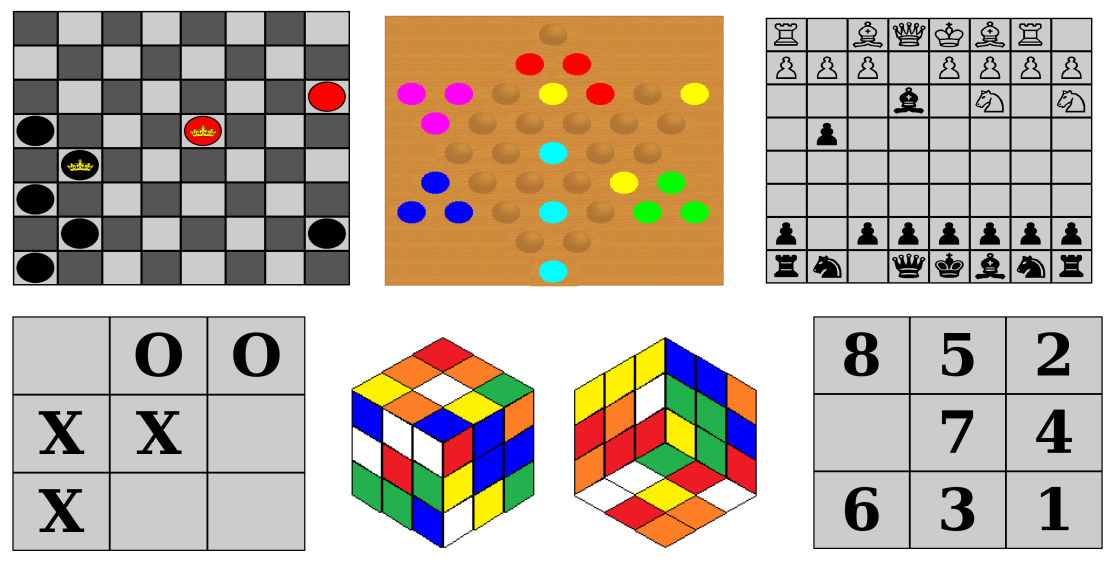
\includegraphics[width=0.7\linewidth]{GGP-Games.png}}
	\caption{A selection of games from the GGP competition. From the top right: \textit{checkers}, \textit{chinese checkers}, \textit{chess}, \textit{tic tac toe}, \textit{rubix cube} and \textit{eight puzzle}}
\end{figure}

\begin{listing}[ht]
\begin{minted}[fontsize=\footnotesize]{text}
(succ 0  1)
(succ 1  2)
(succ 2  3)
(beats scissors paper)
(beats paper stone)
(beats stone scissors)
(<= (legal ?p scissors) (player ?p))
(<= (legal ?p paper) (player ?p))
(<= (legal ?p stone) (player ?p))
(<= (draws ?p) (does ?p ?a) (does ?q ?a) (distinct ?p ?q))
(<= (wins ?p) (does ?p ?a1) (does ?q ?a2) (distinct ?p ?q) (beats ?a1 ?a2))
(<= (loses ?p) (does ?p ?a1) (does ?q ?a2) (distinct ?p ?q) (beats ?a2 ?a1))
\end{minted}
\caption{
\ac{is this listing referenced in the text?}
A sample of rules from the GDL description of Rock Paper Scissors. The $?$ indicates a variable and $<=$ indicates an implication with the first expression after being the head and the conjugation of the rest making up the body
}
\end{listing}


These GDL game descriptions form the basis for the Inductive General Game Playing (IGGP) problem \ac{citation needed}. The task is an inversion of the GGP problem. Rather than taking game rules and using them to play the game in IGGP the aim is to learn the rules from observations of gameplay, similar to how a human might work out the rules of a game by watching someone play it. Cropper et al. define the IGGP problem in their 2019 paper; given a set of gameplay observations the goal is to induce the rules of the game\cite{Cropper/IGGP}. The games used in IGGP are those from the GGP competition problem set, specified in GDL, meaning they are widely varied in complexity.

\af{GIVE EXAMPLE OF IGGP PROBLEM}

An effective way of solving the IGGP problem is a form of machine learning: Inductive Logic Programming (ILP) \ac{citation needed}. In ILP, the learner is tasked with learning logic programs given some background knowledge and a set of values for which the programs are true or false (also expressed in a logical programming language). In the IGGP paper \cite{Cropper/IGGP}, the authors showed through empirical evaluations that ILP systems achieve the best score in this task compared to other machine learning techniques. The ILP system derive a hypothesis, a logic program that when combined with the background knowledge, entails all of the positive and none of the negative examples\cite{Muggleton/ILP}. In the IGGP paper\cite{Cropper/IGGP} it is also shown that the problem is hard for current ILP systems, with on average only 40\% of the rules being learned by the best performing systems.

However, the existing work has limitations. All existing work has assumed that the gameplay being observed is randomly generated. Rather than agents playing to win they simply make moves at random. Often this has the result of the game terminating before it reaches a terminal state due to a cap on trace length or sections of the rule set remaining completely unused. In previous work there has also not been any research done to ascertain the effects that increasing the number of game observation has on the quality of the induced rules. It is unknown weather there is a threshold at which new any new game traces introduced are insignificant. In this paper we use the IGGP framework to evaluate the ability of ILP agents to correctly induce the rules of a game given different sets of gameplay observations - optimal gameplay verses random gameplay as well as combinations of the two. We also vary the number of gameplay traces from which the ILP systems learn.


It is not obvious whether random or optimal gameplay would be best. When learning the rules of chess would a human rather watch moves being made randomly, or a match between two grandmasters? It is not an easy question to answer. Both situations will result in a restricted view of the game, with certain situations never occurring in each one. This is not only a dilemma in the context of learning game rules. For example, teaching a self driving car to navigate roads requires training it on examples of driving. We would clearly not train it on optimal Formula One quality driving and neither would we train it on random movement of the car. The question to be asked is what is the ideal level of training data to use to best teach a system the rules you want it to learn. In this paper, we try to help give some insight into this fundamental question. Specifically, we ask the following research questions:

\begin{description}
\item[Q1] Does varying the quality of game traces influence the ability for learners to solve the IGGP problems? Specifically, does the quality of game play affect predictive accuracy?
\item[Q2] Does varying the amount of game traces influence the ability for learners to solve the IGGP problems? Specifically, does the quality of game play affect predictive accuracy?
\item[Q3] Can we improve the performance of a learner by mixing the quality of traces?
\end{description}

We will train a range of ILP systems that each use a different approach to the problem on different sets of training data. The results for Q1 will be the most interesting as it is not clear what the expected outcome is. Q2 is an \aco{easier}{probably a better word than easier} question to answer, it is generally accepted that for machine learning problems the more training data you have the better the predictive accuracy of the ML system \ac{citation needed}. We ask this question to get some insight into how much the predictive accuracy is affected by the training set size. Often in ILP only a small amount of training data is needed, adding more data may not significantly affect accuracy \cite{Muggleton/ILP}. The third question is an interesting one. Intuitively greater diversity in the training data should give a result closer to the rule that generated the data. However if a learner is trained on random data and only tested on random data we would expect this to perform better than a learner trained on random data then tested on a mix of optimal and random data. This question thus highlights an issue we face: how do we test the learned game rules?

Ideally the generated rules would be compared directly against the rules in the GDL game descriptions. We would take the generated rule and see for what percentage of all possible game states the reference rule and the learned rule gave the same output. Unfortunately we do not have the computational resources to do this with a lot of the games having too many possible states such as checkers which has a state-space complexity of roughly $5.0 \cdot 10^{20}$\cite{Horssen/Checkers} and sudoku which exceeds $6.6 \cdot 10^{21}$\cite{Felgenhauer/Suduko}. Instead we will test the learned programs on both optimal and random data of the same quality used in training. \af{and maybe a combination as well}

We would also expect models trained on the same distribution as they are tested on to perform best since it is generally accepted that the accuracy of a model increases the closer the test data distribution is to the training data distribution \cite{Mitchell/MachineLearing}. However, Gonzales and Abu-Mostafa\cite{Gonzalez/MismatchedOutperform} suggest that a system trained on a different domain to the one it is tested can outperform a system trained and tested on the same domain. Given a test distribution there exsists a duel distribution that, when used to train, gives better results. The duel distribution gives a lower out-of-sample\footnote{out-of-sample data is data that is not in the training set} error than using the test distribution. This duel distribution can be thought of as the point in the input space where the least out-of-sample error occurs\cite{Gonzalez/MismatchedOutperform}. As well as optimising the single training distribution we can take data from multiple distinct distributions. Ben-David et. al. show that training data taken from multiple different domains can in fact give lower error on testing data that traning data taken from any single domain, including the testing domain \cite{Ben-David/DifferentDomains}. It is not clear in our case what selection of training data will result in the most effect learning.

To help answer questions 1-3, we make the following contributions:

\subsubsection{Contributions}
\begin{itemize}
\item We implement a system to play GGP games at (1) random, \af{(2) world-leading}, and (3) optimal levels. (Section \ref{sec:experiments})
\item We transform the GGP traces to IGGP problems
\item We train the ILP systems Metagol, Aleph and ILASP on different combinations of optimal and random data as well as testing them on each individually (Section \ref{sec:experiments})
\item We train the ILP systems on differing amounts of traces and test to ascertain the effect this has on the accuracy of the predicted results
\end{itemize}